\subsection{Verification of the model}

When adding different members with a lot of different devices, the model can become quite complex. Thus, it becomes impossible to verify if the behaviors observed are the expected ones. So before trying to make any results, a set of tests were made to verify that the model of each device works as expected.

\begin{table}[h!]
    \centering
    \begin{tabular}{|c|c|c|c|}
        \hline
        Member & Heating system (thermal load) & Washing machine (white good) & Electric vehicle \\ \hline
        1      & X  &    &    \\ \hline
        2      &   & X &     \\ \hline
        3      &   &  & X   \\ \hline
        4      & X   & X  & X   \\ \hline
    \end{tabular}
    \caption{Members test setup}
    \label{tab:test_members}
\end{table}

The table \ref{tab:test_members} shows the setup of each member in terms of devices. The presence of an "X" in a cell indicates that the corresponding device is present for that member. This way, by putting a production between 10AM and 2PM, we should see that the electric vehicle is charged during this period for member 3, that the washing machine is used during this period for member 2, and that the heating system is used more strongly during this period with sociological profiles of ["economic" : 1, "environmental" : 0, "comfort" : 0.1] (in the following parts, the profiles will be noted as [economic, environmental, comfort], so here it would be [1, 0, 0.1]).

Another test was made to verify the model for the exchanges between the members. For this, we made a community with 2 members, one with a production profile constant equal to 10 and the other without. Both of them have a fixed load of 5. As the selling price is lower than the buying price, with a none 0 coefficient for the economic dimension, we should see that the first member sell its excess production to the second member and not to the grid.

Using these tests, we are able to verify that the model works as expected.

\subsection{Construction of the example}

In order to produce results, an example was built. In this example, we defined the parameters of several devices based on very simple physic models and average power output of the different elements. For example, the power of the heating system is linear with the difference between the indoor and outdoor temperature and comparing to real power consumption figures from a bill we can get a power output of around 100 W/°C. The same was done for other devices. For the production profile, we used an irradiance profile built using PVGIS in December at Villeneuve d'Ascq. 

Then based on a presence at home profile, we can define rules for the consumption of the different devices. If we take again the heating system, when the person is at home, the heating system have a maximum comfort reference temperature which depend on the member. Here this reference can vary between 19 and 22 °C. While when the person is not at home, the heating system have a maximum temperature of 15 °C. This gives a reference consumption profile for the heating system. For the possibility of providing flexibility services, we also define a minimum temperature for when the person is at home (here 18 °C). Of course some devices do not have any flexibility range, for example, the lights are on when the person is at home and it is night, and they are off otherwise.

As shown in \ref{fig:methodo_example}, a function that generate random profiles and a function that allocate to a member different devices randomly were built. This way we can easily generate different examples with different production and consumption profiles. Then, the more fitted members can be chosen to build a community where the optimization will be more interesting. Indeed, if the production profiles is always below the consumption profile, the optimization will not be very interesting as the community will not be able to share energy. The other way around, if every member has a high production and battery storage, then sharing energy will not be useful neither.

\begin{figure}[h]
    \centering
    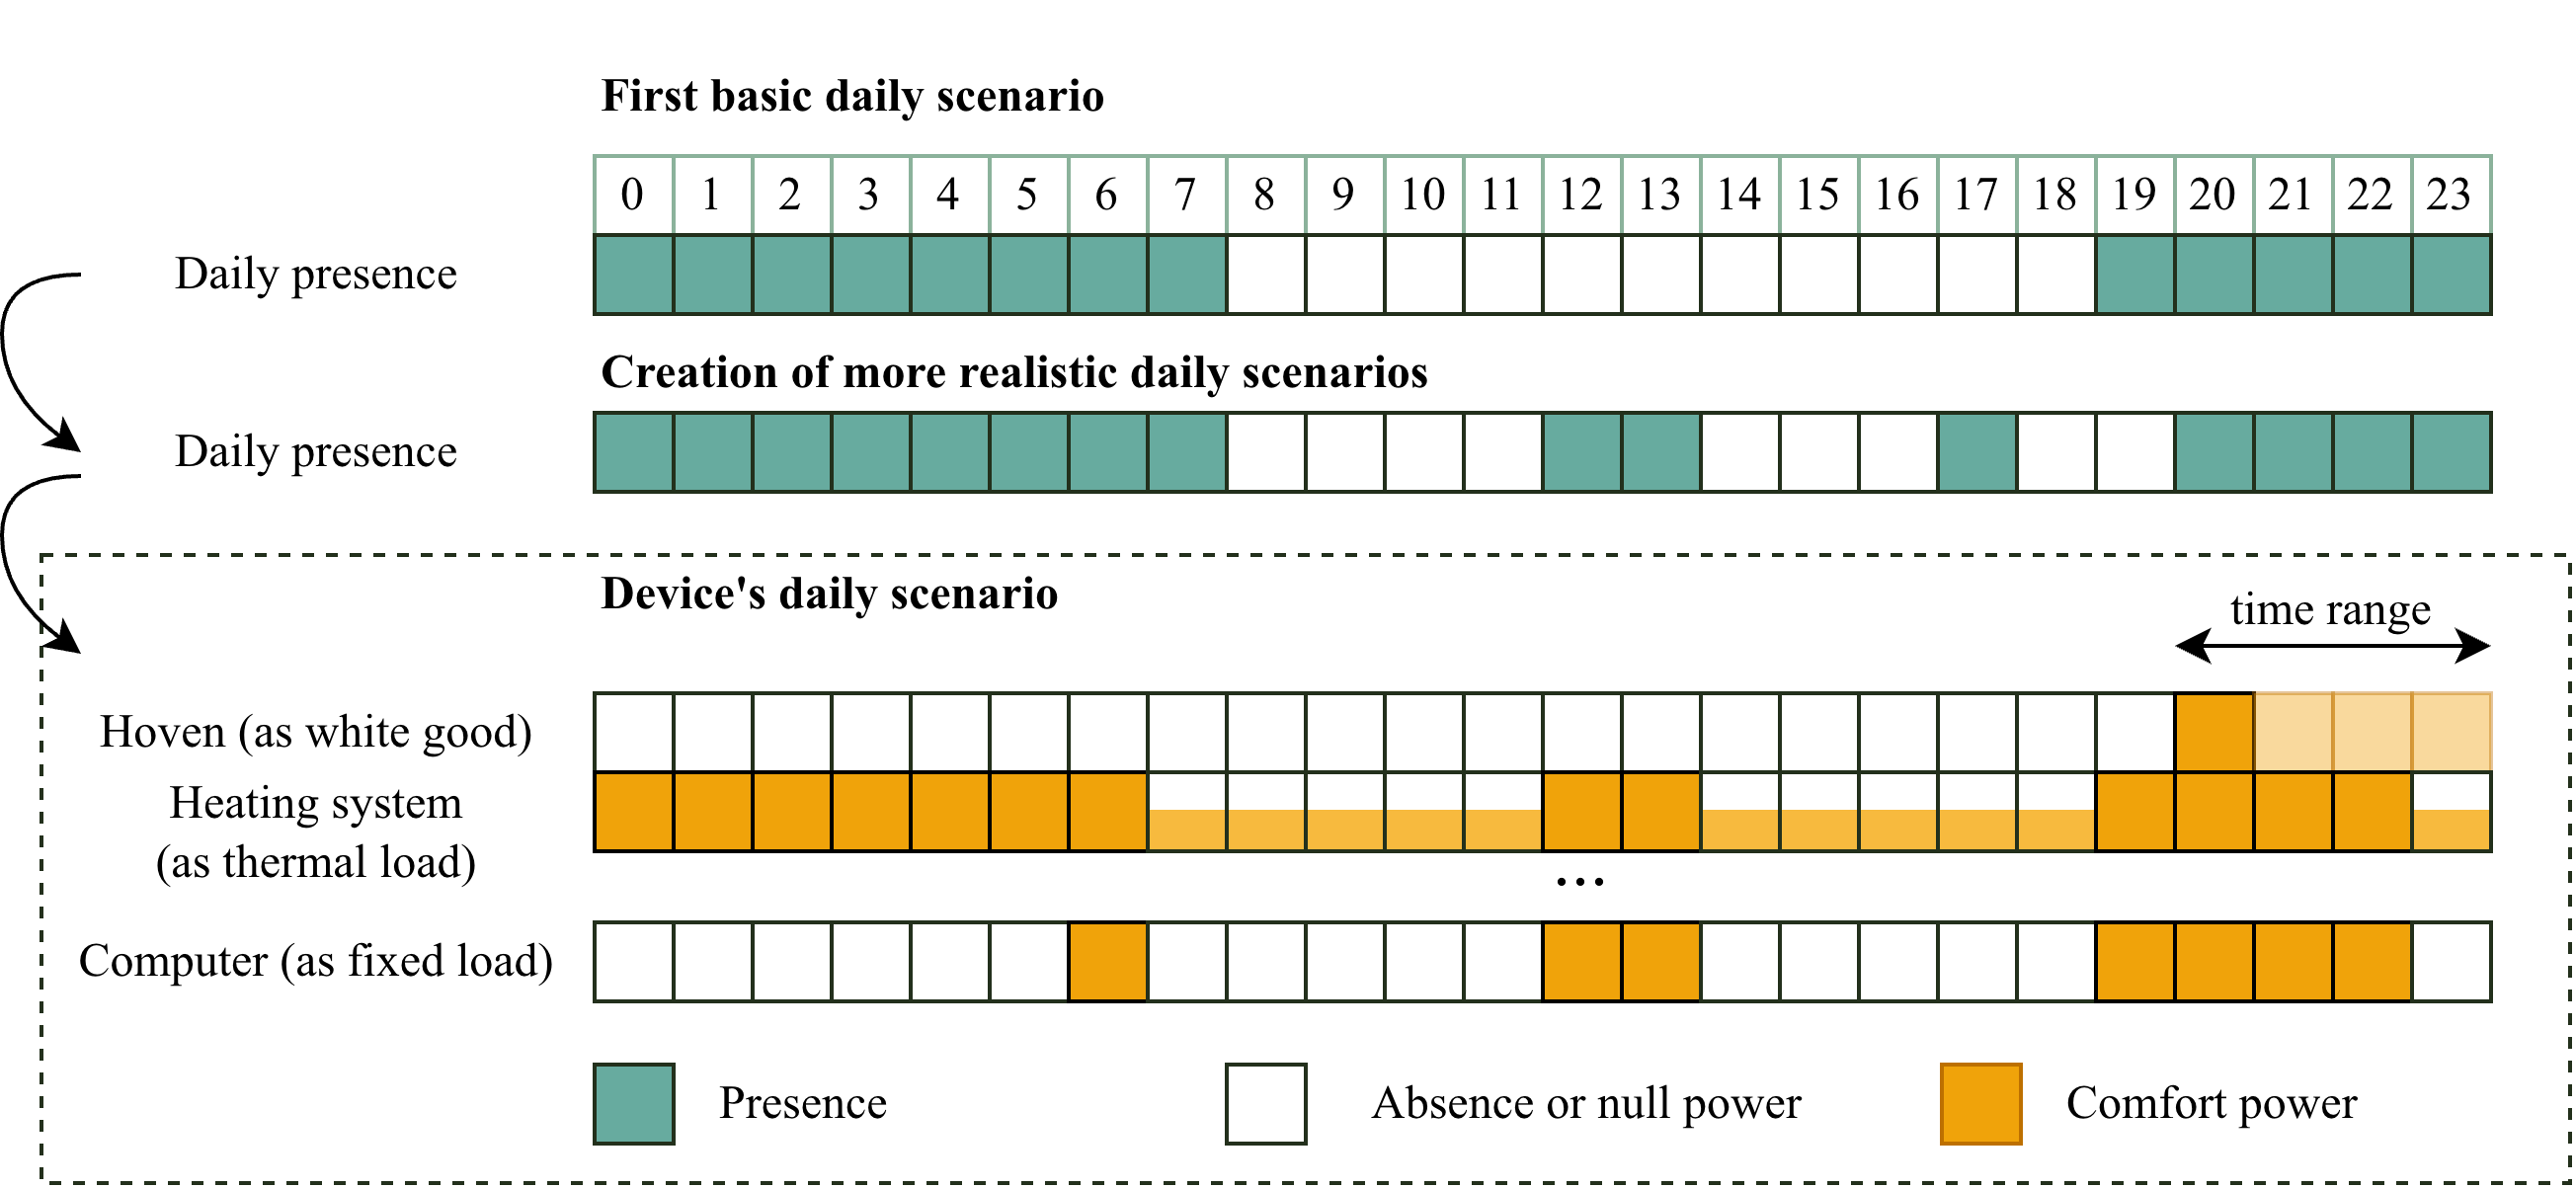
\includegraphics[width=0.7\textwidth]{creation_example.png}
    \caption{Example generation process}
    \label{fig:methodo_example}
\end{figure}

In the end, the community is made of 5 members, so that the results will remain easy to read. The table \ref{fig:table_example} gives the setup of each member of the community in terms of devices. We will then define the sociological profiles based on what we want to show in the different visualizations. Figure \ref{fig:power_profiles_example} shows the power profiles of the different members of the community, for this there are optimized in a fully decentralized way with a sociological profile of [1, 1, 1] for all the members. 


\begin{figure}[!h]
    \centering
    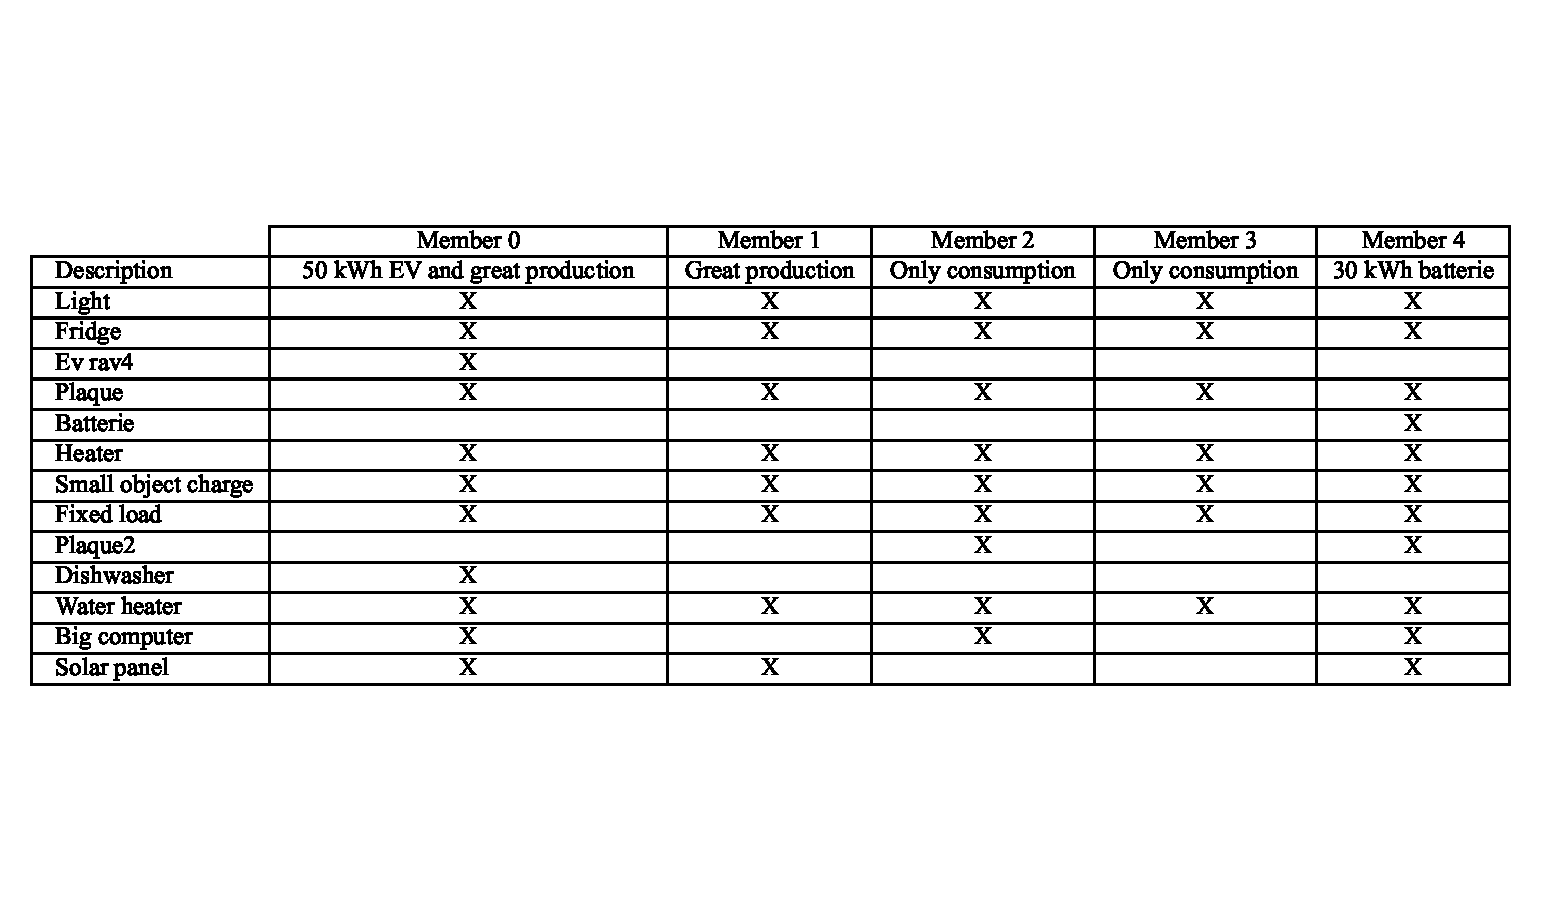
\includegraphics[clip, trim=0cm 4cm 0cm 4cm, width=\textwidth]{dataframe_output.eps}
    \caption{Example setup}
    \label{fig:table_example}
\end{figure}

\newlength{\subfigwidth}
\setlength{\subfigwidth}{0.32\textwidth}
\begin{figure}[h]
    \centering
    \begin{subfigure}[b]{\subfigwidth}
        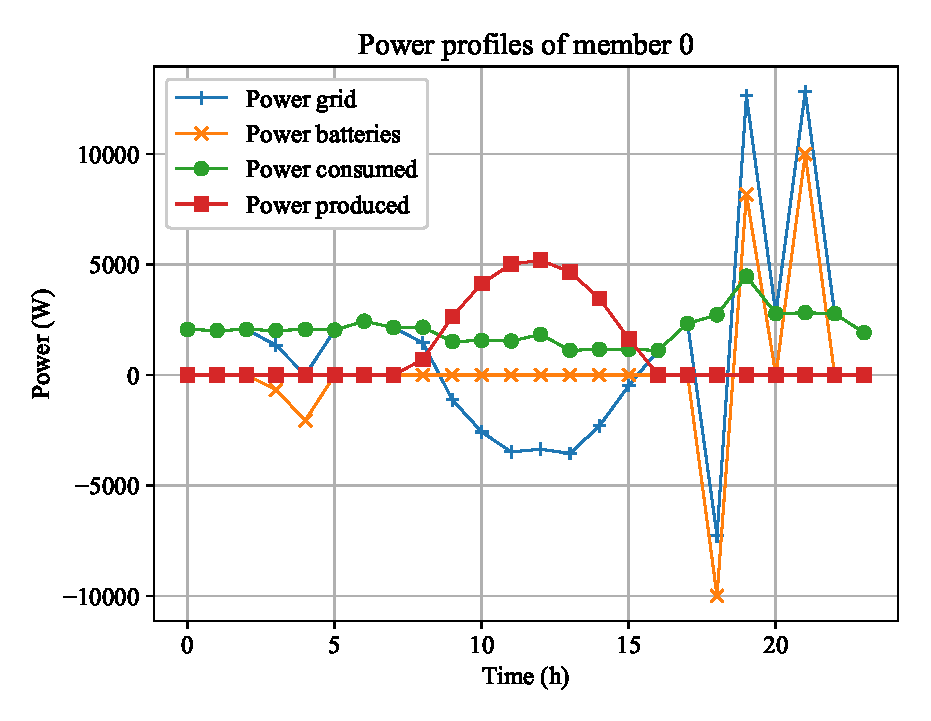
\includegraphics[width=\textwidth]{member_profiles/member_0_power_profiles.eps}
    \end{subfigure}
    \begin{subfigure}[b]{\subfigwidth}
        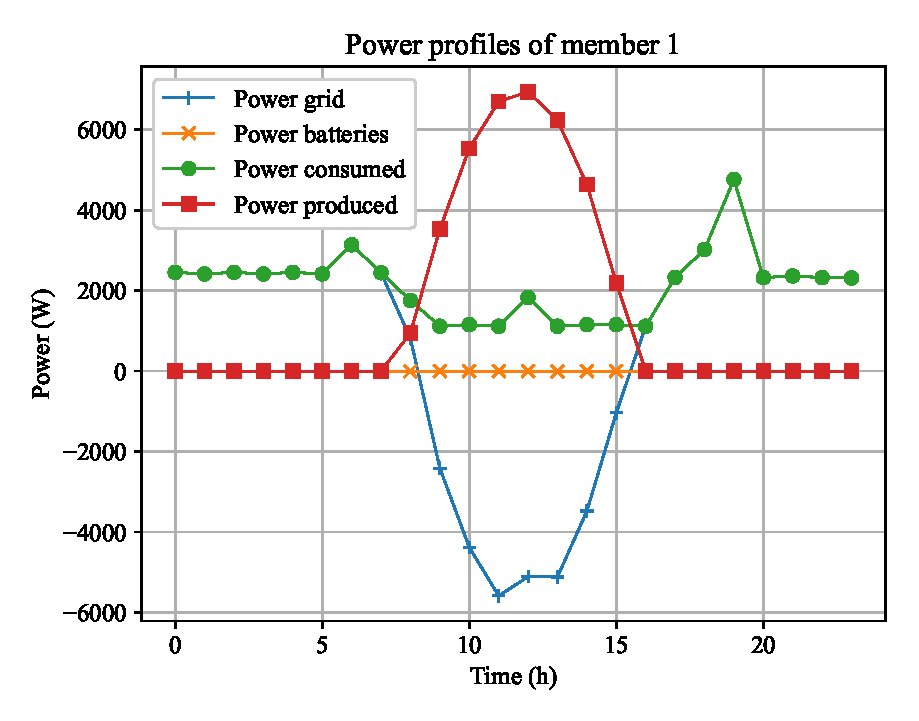
\includegraphics[width=\textwidth]{member_profiles/member_1_power_profiles.eps}
    \end{subfigure}
    \begin{subfigure}[b]{\subfigwidth}
        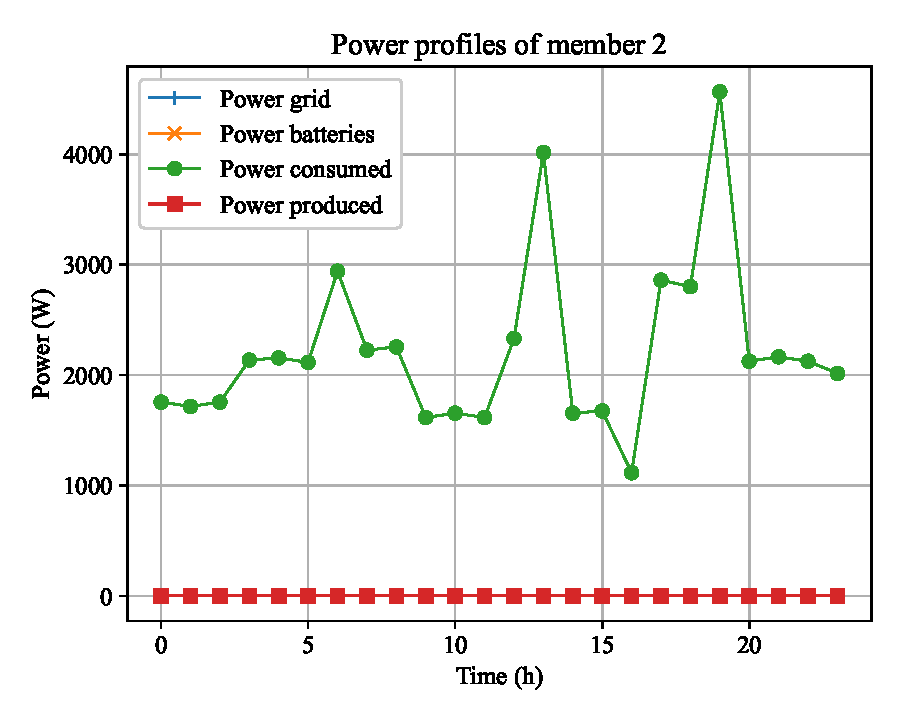
\includegraphics[width=\textwidth]{member_profiles/member_2_power_profiles.eps}
    \end{subfigure}
    \begin{subfigure}[b]{\subfigwidth}
        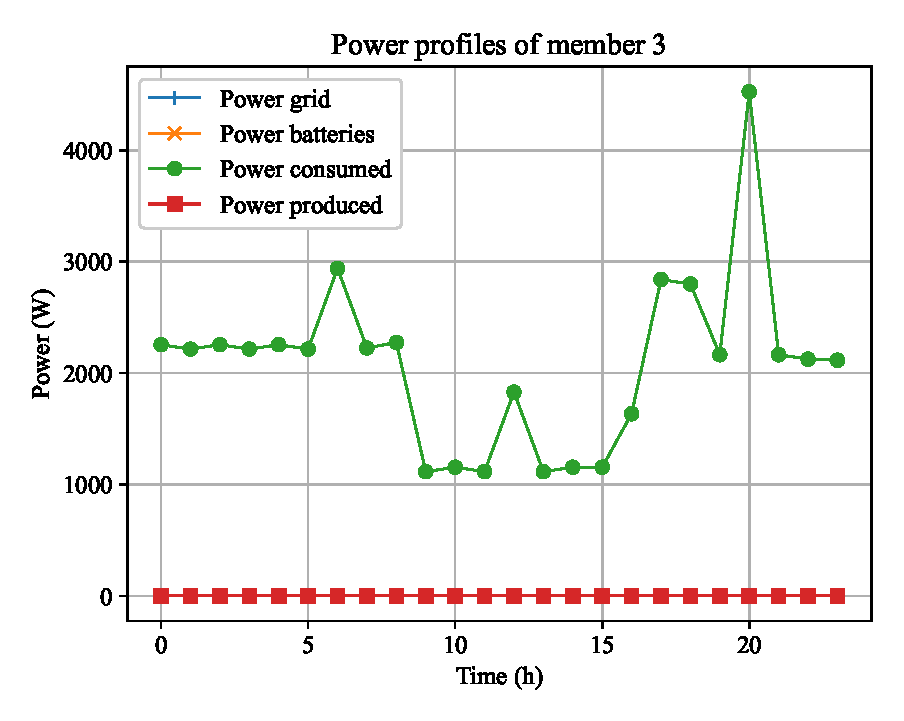
\includegraphics[width=\textwidth]{member_profiles/member_3_power_profiles.eps}
    \end{subfigure}
    \begin{subfigure}[b]{\subfigwidth}
        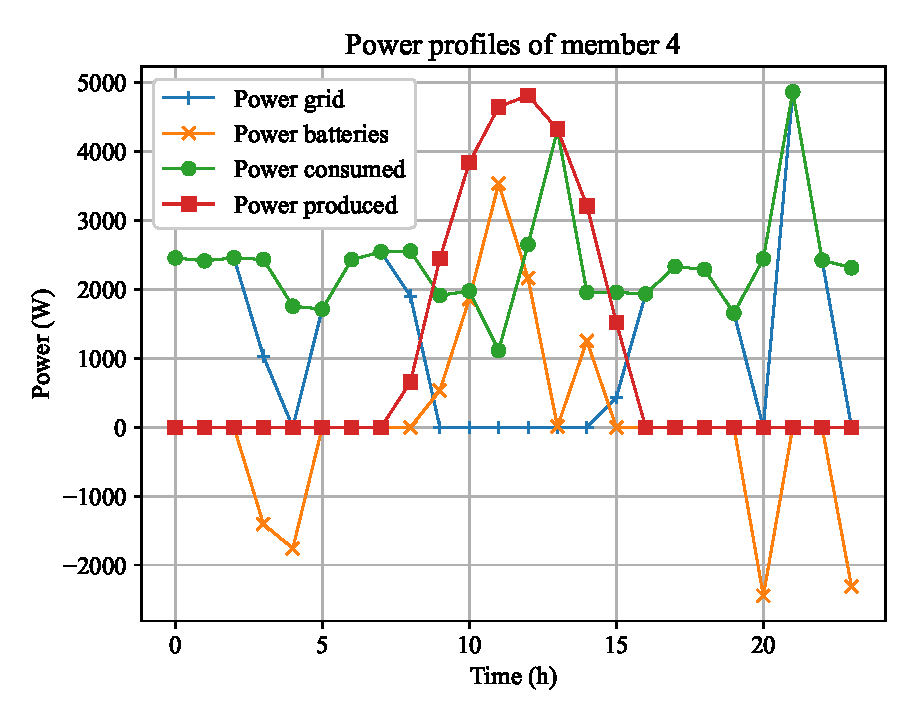
\includegraphics[width=\textwidth]{member_profiles/member_4_power_profiles.eps}
    \end{subfigure}
    \caption{Profile of each member when optimized in a fully decentralized way with a sociological profile of [1, 1, 1] for all the members.}
    \label{fig:power_profiles_example}
\end{figure}
\subsection{Optimization of the community}

With the model of the community built, we can first launch the optimization in a fully decentralized way with a sociological profile equal to [1, 1, 1] for all the members just to look at the behavior of the system. Figure \ref{fig:community_centralized} shows that at midday, the production being a lot higher than the consumption, there is a lot more exchanges withing the community and the batteries are charging. Outside of this, it is quite hard to understand specifically what is happening. Though, we can compare it with the operation when we have different sociological profiles. Figure \ref{fig:diff_profiles} shows the operation of the community with a sociological profile of [1, 0, 0], [0, 1, 0] and [0, 0, 1] for all the members. We can see here, that between the economic only profile and the environmental only one there are some differences, but still, they are quite similar. With the comfort only profile, the model does not care about the community and just maximize the consumption at the wanted time and power output. But it is still hard to interpret what will be the effect of the sociological profile on the operation.

\begin{figure}[!h]
    \centering
    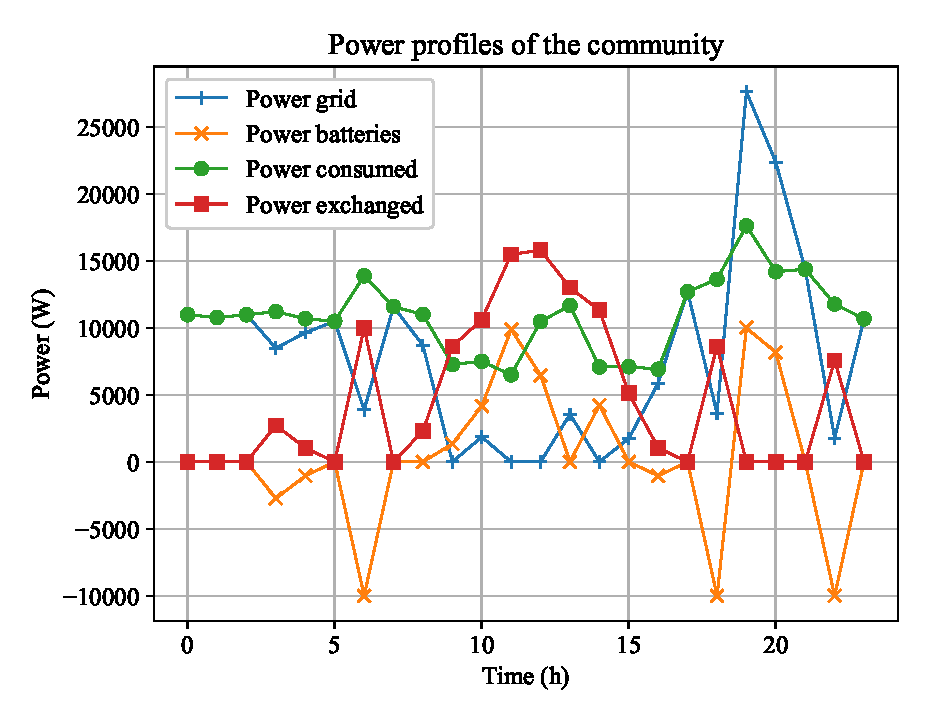
\includegraphics[width=0.48\textwidth]{community_centralized.eps}
    \caption{Operation of the community optimized in a fully centralized way with a sociological profile of [1, 1, 1] for all the members.}
    \label{fig:community_centralized}
\end{figure}

\begin{figure}[!h]
    \centering
    \begin{subfigure}[b]{0.32\textwidth}
        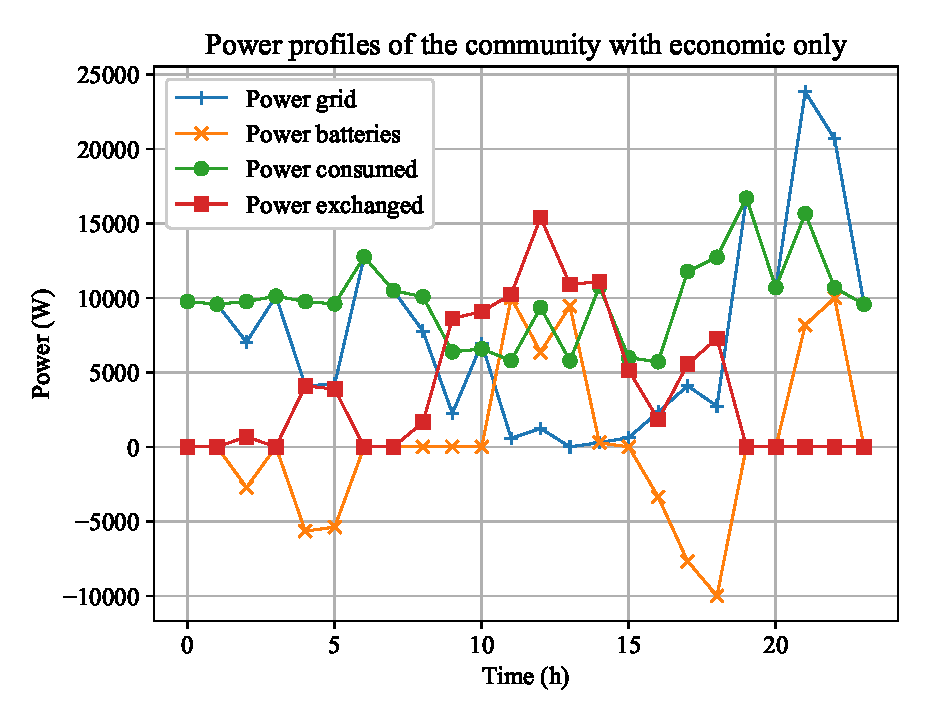
\includegraphics[width=\textwidth]{community_profiles/community_economic_only_power_profiles.eps}
        \caption{Sociological profile [1, 0, 0]}
    \end{subfigure}
    \begin{subfigure}[b]{0.32\textwidth}
        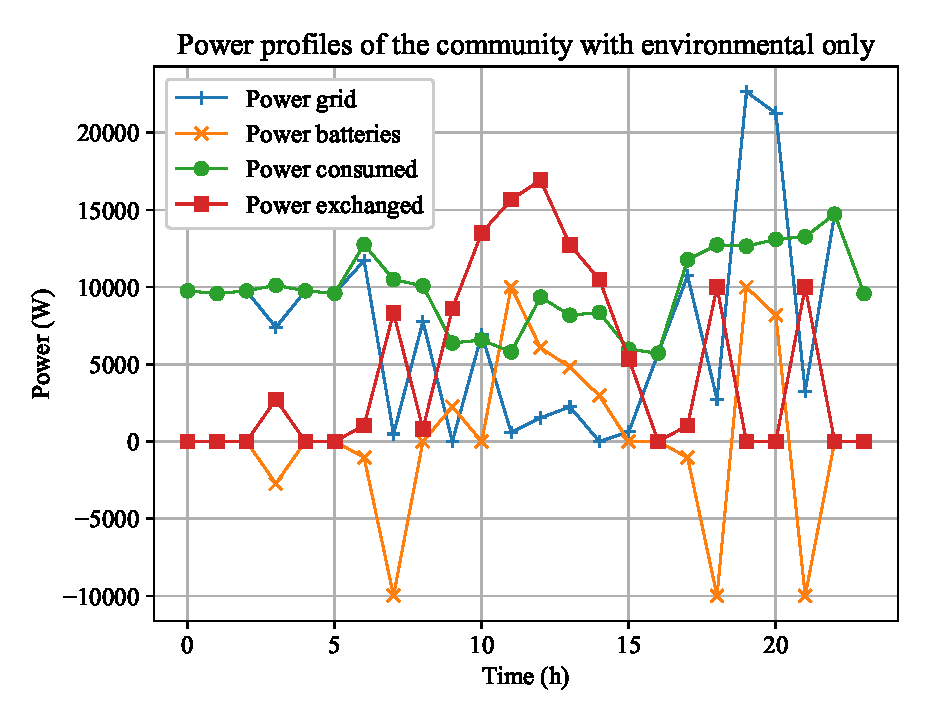
\includegraphics[width=\textwidth]{community_profiles/community_environmental_only_power_profiles.eps}
        \caption{Sociological profile [0, 1, 0]}
    \end{subfigure}
    \begin{subfigure}[b]{0.32\textwidth}
        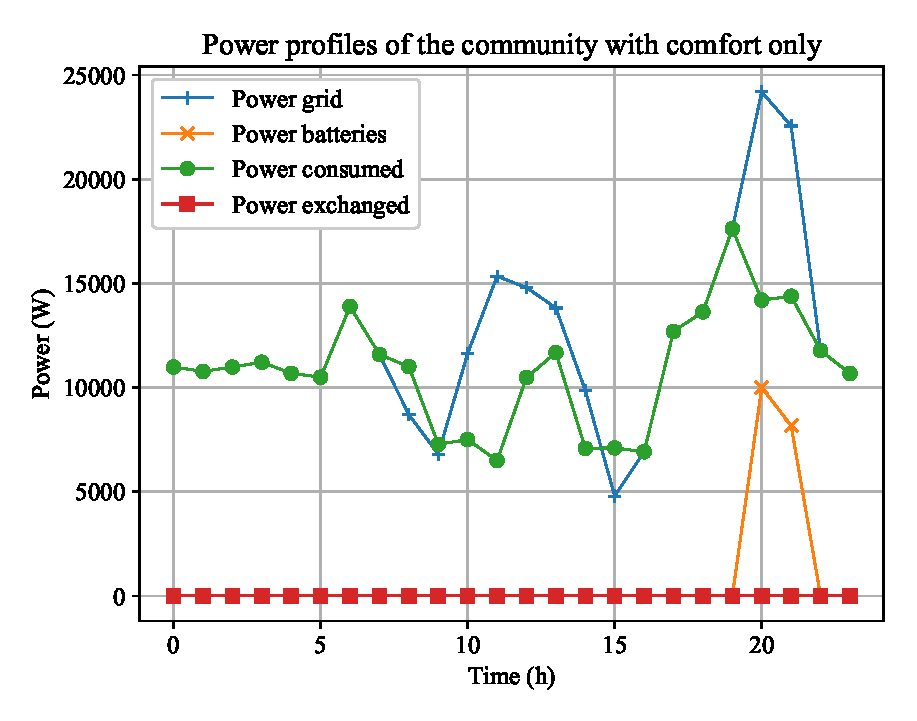
\includegraphics[width=\textwidth]{community_profiles/community_comfort_only_power_profiles.eps}
        \caption{Sociological profile [0, 0, 1]}
    \end{subfigure}
    \caption{Operation of the community with different sociological profiles.}
    \label{fig:diff_profiles}
\end{figure}



So now we will plot the Pareto front of the community by optimizing the community with different sociological profiles. To be able to compare efficiently the values in the Pareto front, it is plotted with the normalized values as explained in \ref{objective_function}. Figure \ref{fig:pareto_front} shows the 3D Pareto front of the community with the different sociological profiles. To understand better, we can also plot the 2D projections \ref{fig:pareto_front_2d}.

\begin{figure}[h]
    \centering
    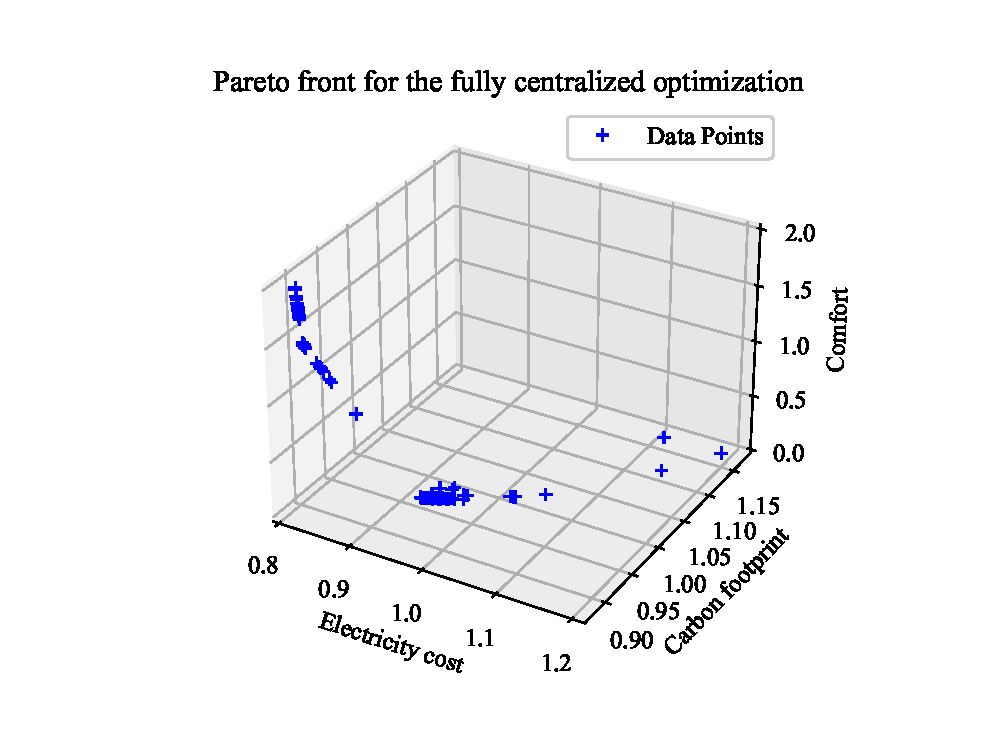
\includegraphics[width=0.8\textwidth]{commu_pareto_front.eps}
    \caption{3D Pareto front of the community with different sociological profiles.}
    \label{fig:pareto_front}
\end{figure}

\begin{figure}[h]
    \centering
    \begin{subfigure}[b]{0.32\textwidth}
        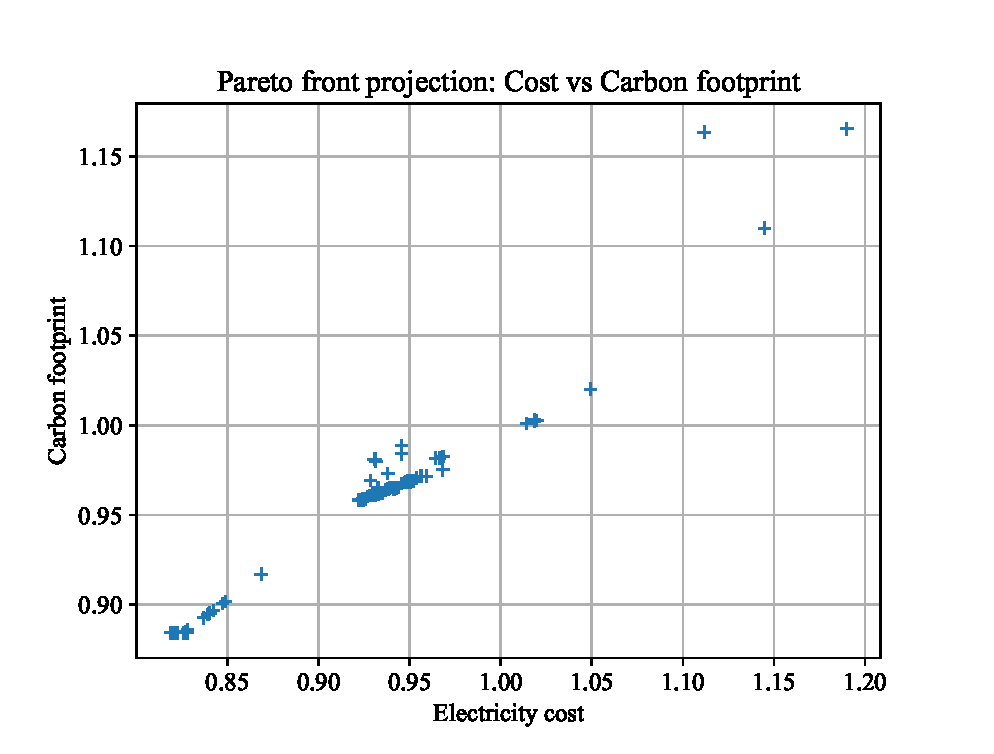
\includegraphics[width=\textwidth]{commu_pareto_front_cost_enviro.eps}
        \caption{Economic vs Environmental}
    \end{subfigure}
    \begin{subfigure}[b]{0.32\textwidth}
        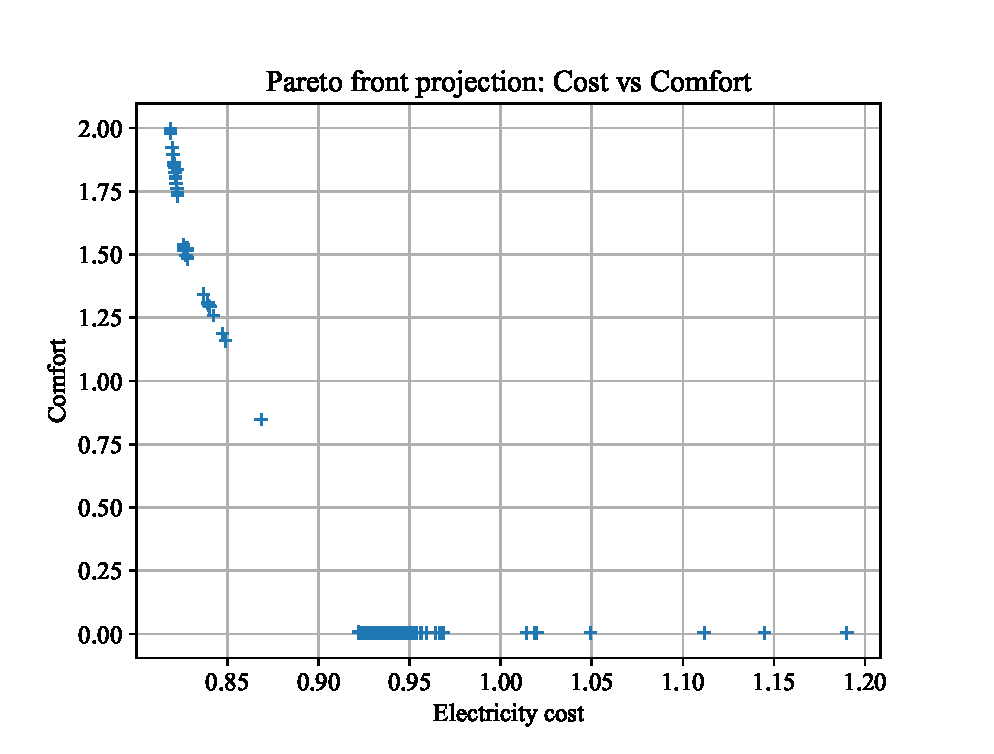
\includegraphics[width=\textwidth]{commu_pareto_front_cost_comfort.eps}
        \caption{Economic vs Comfort}
    \end{subfigure}
    \begin{subfigure}[b]{0.32\textwidth}
        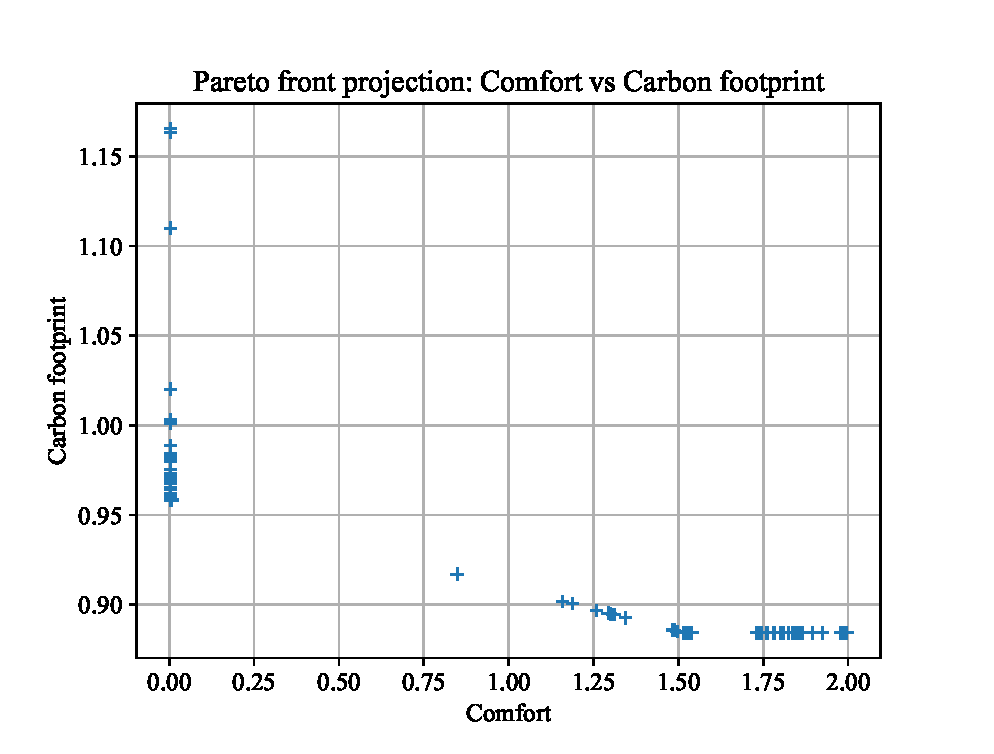
\includegraphics[width=\textwidth]{commu_pareto_front_comfort_enviro.eps}
        \caption{Comfort vs Environmental}
    \end{subfigure}
    \caption{2D projections of the Pareto front of the community with different sociological profiles.}
    \label{fig:pareto_front_2d}
\end{figure}

As we could have imagined while defining the objective function, there is a strong correlation between optimizing the environmental cost and the economic cost. Indeed, for both of them the cost is lower when we maximize the self consumption of the community. So the analysis between the comfort and the economic cost will be the same as between the comfort and the environmental cost. 

In the model, there is a minimum and a maximum comfort possible. The interesting part of the curve is thus the one where the comfort value is not yet at its maximum. And we can see that there is a clear trade-off between the comfort and the economic/environmental cost. The minimum economic cost for a comfort cost of 0 is around 0.92, while the minimum economic cost is around 0.82. Meaning a decrease of 11\%. The value is the same for the environmental cost. Of course this value depends a lot on the bounds we set, but the slopes of the curve can give us good insight on this trade-off. Another important point is that here the sociological profile of the community is computed as the average of the sociological profile of the members. So the trade-off to find will be between every member of the community.

Maybe a model involving the dimensioning of the production and storage capacities of the community would be more interesting for studying the Pareto Front as we should have more complex interactions between the price and the environmental cost. The model developed here could be improved for this by adding some variables and constraints.

\subsection{Gain allocation}

Now that we have seen the behavior of this community model, we will explore the gain allocation. For this, we will define some profiles for the members of the community as shown in \ref{tab:profiles}. They have been built in order to have a good variety of profiles in the community. The profile of the community is computed as the average of the profiles of the members. 

\begin{table}[h]
    \centering
    \begin{tabular}{|c|c|c|c|}
        \hline
        Member & Economic & Environmental & Comfort \\ \hline
        0      & 0.4  & 0.1  & 0.5     \\ \hline
        1      & 0.5  & 0.2  & 0.3     \\ \hline
        2      & 0.8  & 0.1  & 0.1     \\ \hline
        3      & 0.4  & 0.4  & 0.2     \\ \hline
        4      & 0.2  & 0.6  & 0.2     \\ \hline
        Community & 0.46 & 0.28 & 0.22    \\ \hline
    \end{tabular}
    \caption{Sociological profiles of the members of the community}
    \label{tab:profiles}
\end{table}

In this set-up, there is and economic gain of 15\% by participating in the community. In the figure \ref{fig:gain_allocation_radar}, we can see the comparison between each method.

\begin{figure}[h]
    \centering
    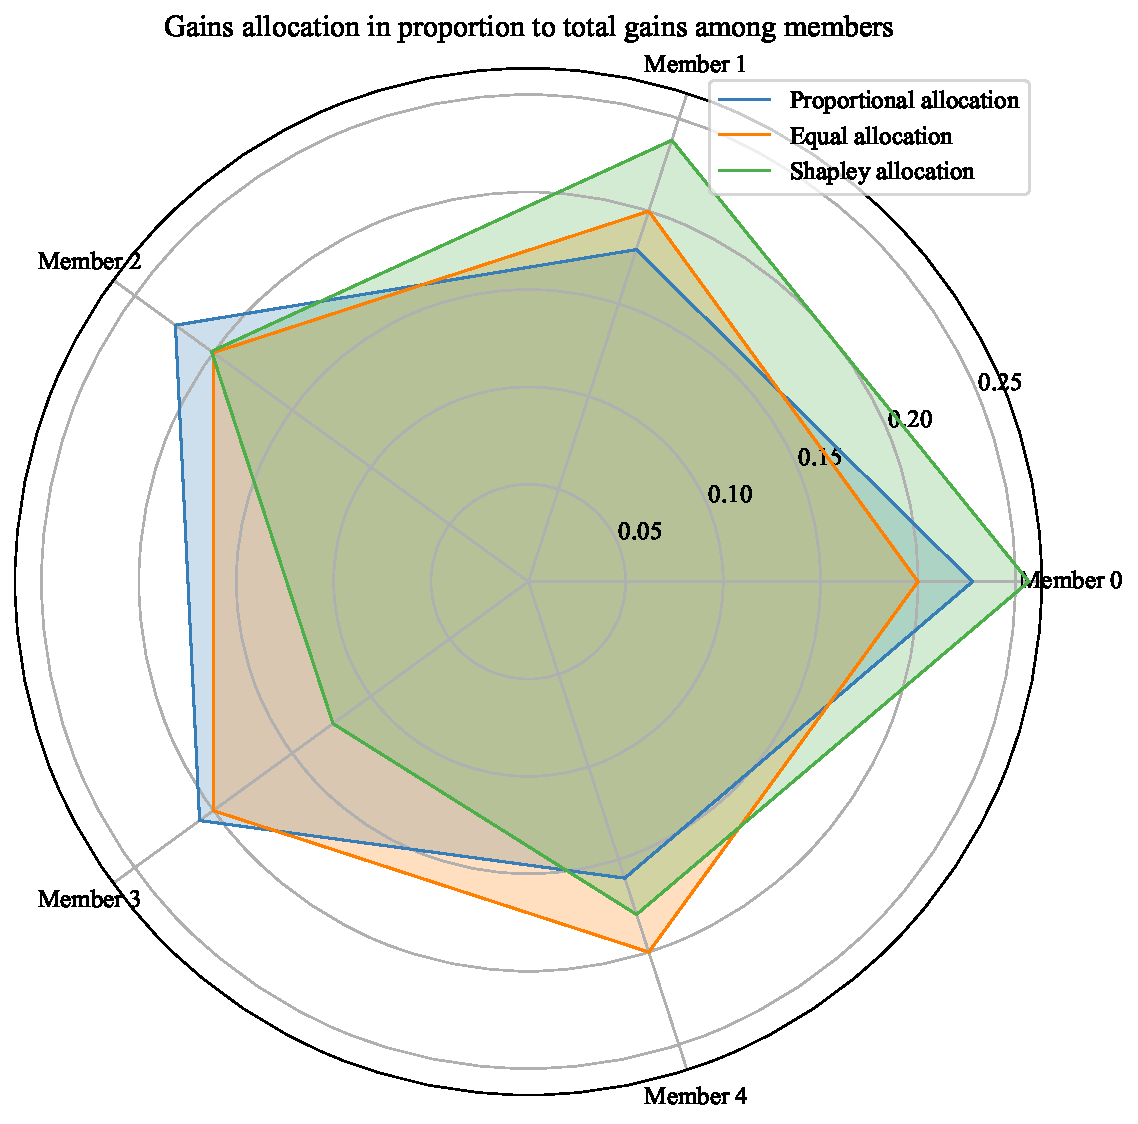
\includegraphics[width=0.5\textwidth]{gains_allocation/gains_allocation_proportional.pdf}
    \caption{Gains allocation in proportion to total gains among members.}
    \label{fig:gain_allocation_radar}
\end{figure}

Each method is not allocating the gain towards the same members. Here we can use the equal allocation as a reference in order to understand which members are favored by the different methods. The Shapley value gives more gain to members 0 and 1, a bit less to 2. Again a bit less to 4 and a lot less to 3. The proportional allocation is more equal by giving a bit more gain to 0, 2 and 3, and a bit less to 1 and 4.

One thing important to understand is that both methods have real mathematic arguments to be used. The Shapley value is a method that is based on the contribution of each member to the gain of the community, while the proportional allocation is a method that is based on the contribution of each member to the cost reduction of the community. But using one or the other result in differences in the gain allocation. To understand these results better we can compare the gain allocation with the resources of each member. Figure \ref{fig:gain_allocation_resources} shows each allocation compared to the installed production rate as well as the battery capacity rate and the consumption rate of each member.

\begin{figure}[!h]
    \centering
    \begin{subfigure}[b]{0.48\textwidth}
        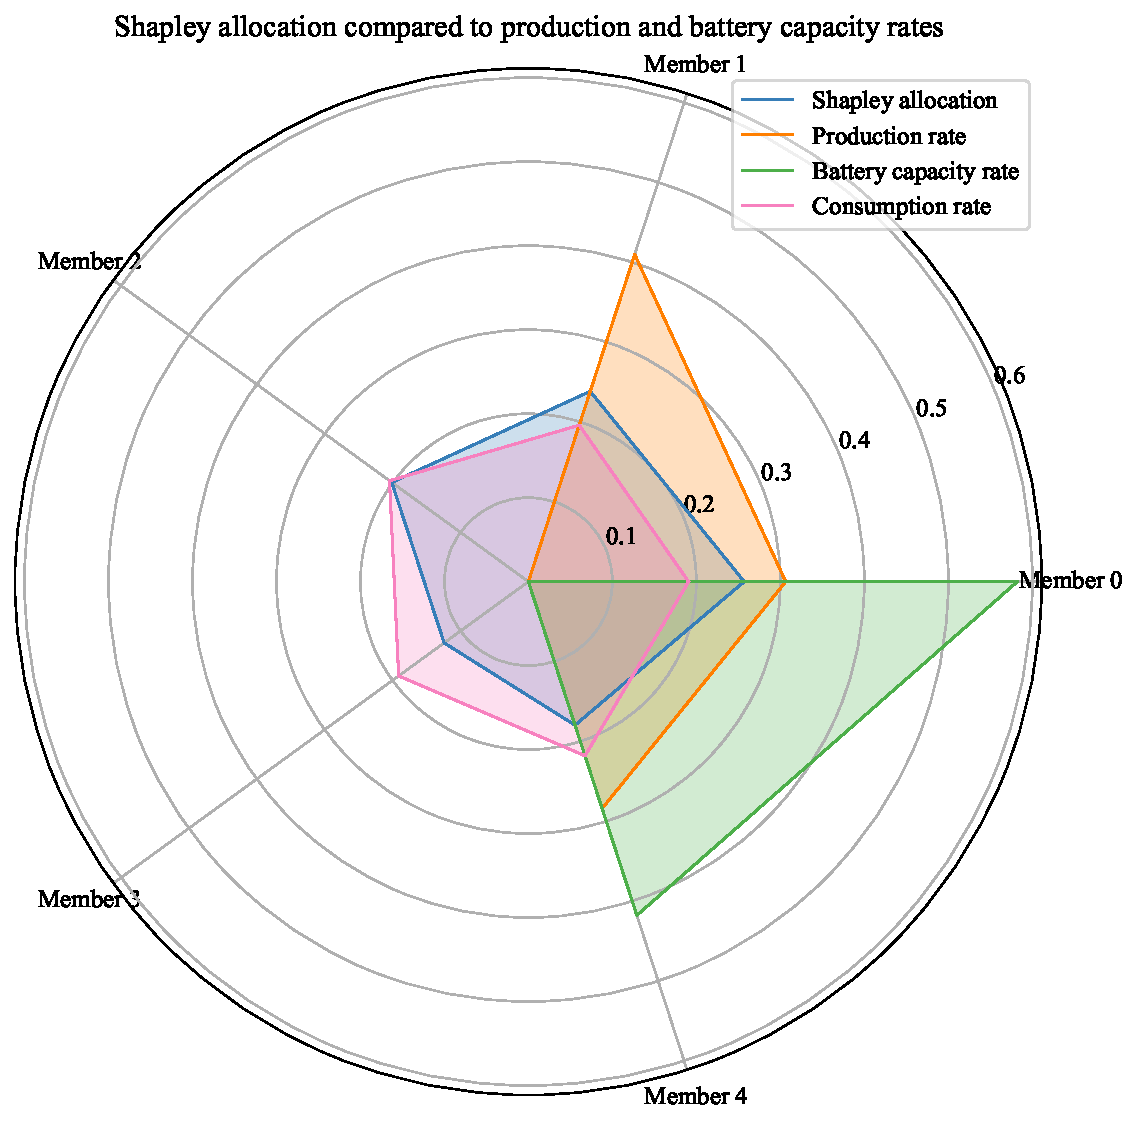
\includegraphics[width=\textwidth]{gains_allocation/shapley_vs_production_battery.pdf}
        \caption{Proportional allocation compared to the resources of each member.}
    \end{subfigure}
    \begin{subfigure}[b]{0.48\textwidth}
        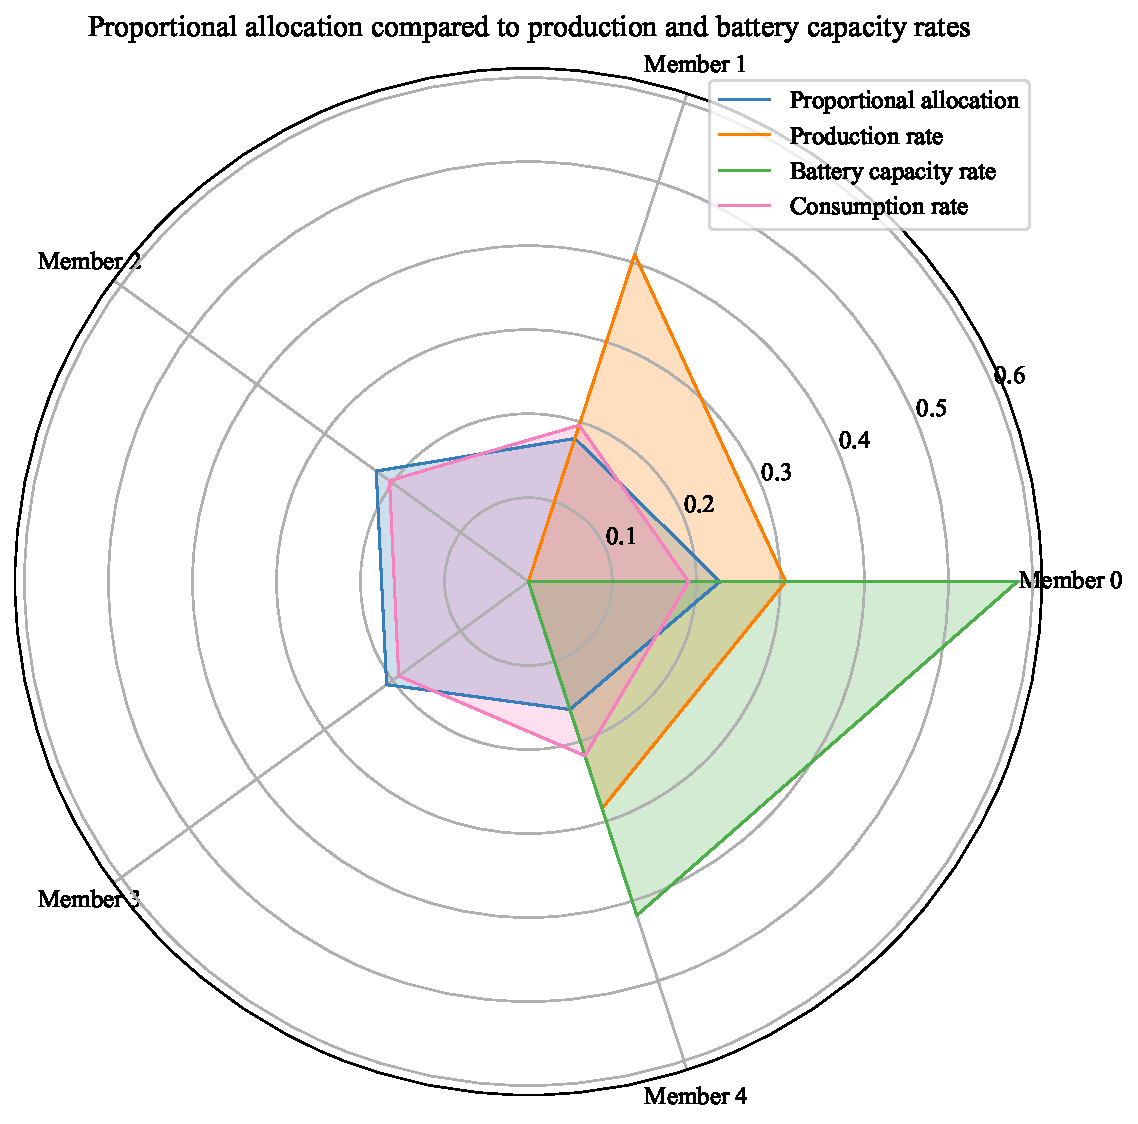
\includegraphics[width=\textwidth]{gains_allocation/proportional_vs_production_battery.pdf}
        \caption{Shapley allocation compared to the resources of each member.}
    \end{subfigure}
    \caption{Comparison of the gain allocation with the resources of each member.}
    \label{fig:gain_allocation_resources}
\end{figure}

The first thing we notice is that the consumption is almost equal for all members but member 4 which have a slightly higher consumption. Then as explained in the construction of the example, only member 0 and 4 have a battery capacity, and the one from 4 is available all day while the one from 0 is not available at midday. Finally, three members have a production, and the one from member 1 is higher than the two others. 

With this being said, the Shapley value works as expected in a meritocratic way by giving more gain to the members with solar production. But the consumption profile is also important. Indeed, we could think that member 4 would receive more as they have production and a battery storage. But having a higher consumption, they do not participate so much in reducing the objective cost of the community, and thus they do not receive a lot of gain. This behavior could bring some fairness problematics as the member 4 might receive less gain than member 2 for example, while he invested much more.

In the case of the proportional allocation, it seems hard to understand without understanding mathematically how the gain is computed. Indeed, two of the members receiving more gain than the others do not have any production. While, two of the members receiving less gain than the others have a production. This is because the gain is computed based on the cost reduction of the community as whole. So using this method that is supposed to reach Nash equilibrium, i.e. a state where no member can do better by changing its strategy while the other members keep their strategy unchanged, can lead to result that are not fair in a meritocratic way. It can be seen as a "max-min" fairness allocation function.

Of course the equal allocation is the most egalitarian one, it does not take into account the contribution of each member to the gain of the community at all. 

